\documentclass[a4paper,DIV=13,11pt,UKenglish,titlepage=firstiscover,abstract=on]{scrreprt}
\usepackage[style = nature, abbreviate = true, doi = true, backend = biber]{biblatex}
\usepackage[onehalfspacing]{setspace}
\usepackage{graphicx}
\usepackage{times}
\usepackage{csquotes}
\usepackage[UKenglish]{babel}
\usepackage[textsize=tiny]{todonotes}
\usepackage[acronym]{glossaries}
\usepackage{soul} % for command \hl
\usepackage{pdfpages} % to insert pdf docs
\usepackage{csvsimple} % to import .csv files as tables
\usepackage{tikz}
\usepackage{float}
\usepackage{tikz}
% from seminar template
\usepackage[T1]{fontenc}       % andere Schriftsatzkodierung für richtige Silbentrennung bei Umlauten
\usepackage{lmodern}           % Vektorschriftarten für besseres pdf
\usepackage{amsmath}           % Verbesserte Mathematikumgebungen
\usepackage[per-mode=symbol-or-fraction,output-decimal-marker={,}]{siunitx} % für das korrekte und einfache Setzen von Einheiten
\usepackage{color}             % falls farbiger Text benötigt wird
\usepackage{wrapfig}           % für Bilder, die nicht die ganze Seitenbreite einnehmen sollen
\usepackage[format=plain,font=small,labelfont=bf]{caption} % Formatierung der Beschriftungen (insbesondere für umfließend gesetzte Bilder wichtig)
\usepackage[pdfauthor={AutorIn Name},pdftitle={Sehr interessanter Titel},pdfsubject={Bachelorarbeit 2022S.705.615}]{hyperref}        % für Hyperlinks und pdf-Metadaten
\linespread{1.125} % Zeilenabstands- und Schriftartoptionen, für weitere Informationen bitte die Anleitung scrguide.pdf für die KOMA-Script Klassen lesen



\AtBeginBibliography{\small}
\addbibresource{main_sources.bib}

\setlength{\parindent}{0cm}

\setlength{\marginparwidth}{3.5cm} % make todonotes wider
\newcommand{\todoleft}[1]{{\reversemarginpar \todo{#1}}}


%%%%%%%%%%%%%%%%%%%%%%%%%%%%%%%%%%%%%%%%%%%%%%%%%%%%%%%%%%%%%%%%%%
\begin{document}
\def\findate{\today}


%title page
\thispagestyle{empty}
\begin{center}
    \Large{University of Innsbruck \\ Faculty of Mathematics, Computer Science and Physics} \\
    \vspace{3mm}
    \large{Institute for Theoretical Physics}
    \vspace{10mm}

    \includegraphics[width = 0.6 \linewidth]{logo.jpg}

    \vspace{10mm}
    \Large{Bachelor Thesis} \\
    \large{submitted for the degree of} \\
    \Large{Bachelor of Science} \\
    \vspace{10mm}
    \LARGE{\textbf{An Information-Theoretical Approach to Internal Models in a Partially Observable Markov Decision Process}} \\
    \vspace{10mm}

    \large{by \\ Lukas Prader \\ Matriculation Nr.: 12115058}
\end{center}

\vspace{30mm}
\begin{tabular}{ll}
    \large{Submission Date:} & \large{\findate}                          \\
    \large{Supervisors:}     & \large{Alexander Vining, Hans J  Briegel} \\
\end{tabular}


\newpage
\thispagestyle{empty}
\begin{abstract}
    Lorem ipsum
\end{abstract}

\pagenumbering{roman}

\tableofcontents

\clearpage
\pagenumbering{arabic}

\chapter{Introduction} \label{chap:introduction}


\chapter{Results} \label{chap:results}

\section{Markov Process Plots}

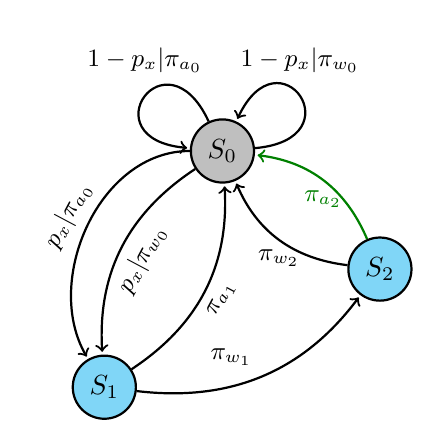
\begin{tikzpicture}[->,shorten >=1pt,auto,node distance=3cm,
        thick,main node/.style={circle,draw,font=\sffamily\Large\bfseries}]

    \node[fill=gray!50, circle, draw=black] (0) at (0,0) {$S_0$};
    \node[fill=cyan!50, circle, draw=black] (1) at (-1.5,-3) {$S_1$};
    \node[fill=cyan!50, circle, draw=black] (2) at (2,-1.5) {$S_2$};

    \path[every node/.style={font=\sffamily\small}]
    (0) edge [in=175,out=115, loop] node[above=5pt] {$1-p_x | \pi_{a_0}$} (0)
    (0) edge [in=65,out=5, loop] node[above=5pt] {$1-p_x | \pi_{w_0}$} (0)
    (0) edge [in=120,out=180] node[above, rotate=62] {$p_x | \pi_{a_0}$} (1)
    (0) edge [bend right] node[below, rotate=62] {$p_x | \pi_{w_0}$} (1)
    (1) edge [bend right] node[below, rotate=62] {$\pi_{a_1}$} (0)
    (1) edge [bend right] node {$\pi_{w_1}$} (2)
    (2) edge [bend left] node[below] {$\pi_{w_2}$} (0)
    (2) edge [bend right, black!50!green] node[below] {$\pi_{a_2}$} (0);

\end{tikzpicture}

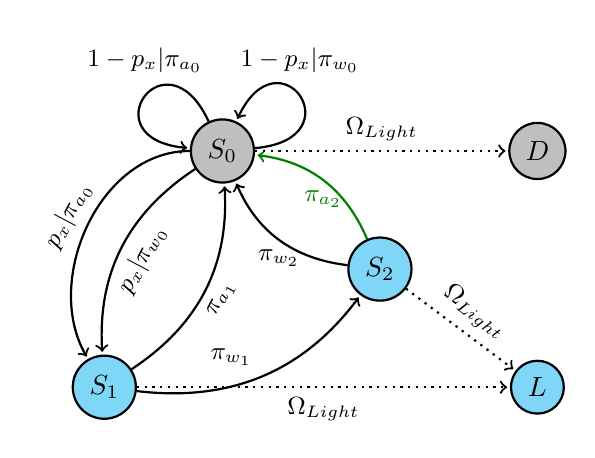
\begin{tikzpicture}[->,shorten >=1pt,auto,node distance=3cm,
        thick,main node/.style={circle,draw,font=\sffamily\Large\bfseries}]

    \node[fill=gray!50, circle, draw=black] (0) at (0,0) {$S_0$};
    \node[fill=cyan!50, circle, draw=black] (1) at (-1.5,-3) {$S_1$};
    \node[fill=cyan!50, circle, draw=black] (2) at (2,-1.5) {$S_2$};
    \node[fill=gray!50, circle, draw=black] (D) at (4,0) {$D$};
    \node[fill=cyan!50, circle, draw=black] (L) at (4,-3) {$L$};

    \path[every node/.style={font=\sffamily\small}]
    (0) edge [in=175,out=115, loop] node[above=5pt] {$1-p_x | \pi_{a_0}$} (0)
    (0) edge [in=65,out=5, loop] node[above=5pt] {$1-p_x | \pi_{w_0}$} (0)
    (0) edge [in=120,out=180] node[above, rotate=62] {$p_x | \pi_{a_0}$} (1)
    (0) edge [bend right] node[below, rotate=62] {$p_x | \pi_{w_0}$} (1)
    (1) edge [bend right] node[below, rotate=62] {$\pi_{a_1}$} (0)
    (1) edge [bend right] node {$\pi_{w_1}$} (2)
    (2) edge [bend left] node[below] {$\pi_{w_2}$} (0)
    (2) edge [bend right, black!50!green] node[below] {$\pi_{a_2}$} (0)
    (0) edge [dotted] node[above] {$\Omega_{Light}$} (D)
    (1) edge [dotted] node[below] {$\Omega_{Light}$} (L)
    (2) edge [dotted] node[above, rotate=-38] {$\Omega_{Light}$} (L);

\end{tikzpicture}

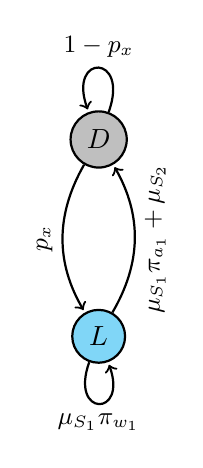
\begin{tikzpicture}[->,shorten >=1pt,auto,node distance=3cm,
    thick,main node/.style={circle,draw,font=\sffamily\Large\bfseries}]

\node[fill=gray!50, circle, draw=black] (D) at (4,0) {$D$};
\node[fill=cyan!50, circle, draw=black] (L) at (4,-2.5) {$L$};

\path[every node/.style={font=\sffamily\small}]
(D) edge [in=110,out=70, loop] node[above] {$1-p_x$} (D)
(D) edge [bend right] node[above, rotate=90] {$p_x$} (L)
(L) edge [bend right] node[below, rotate=90] {$\mu_{S_1}\pi_{a_1} + \mu_{S_2}$} (D)
(L) edge [in=290,out=250, loop] node[below] {$\mu_{S_1}\pi_{w_1}$} (L);

\end{tikzpicture}

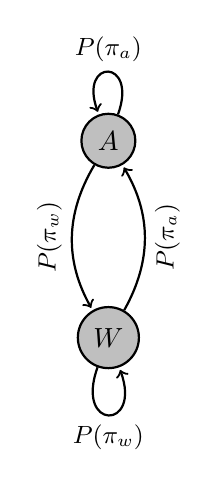
\begin{tikzpicture}[->,shorten >=1pt,auto,node distance=3cm,
    thick,main node/.style={circle,draw,font=\sffamily\Large\bfseries}]

\node[fill=gray!50, circle, draw=black] (A) at (4,0) {$A$};
\node[fill=gray!50, circle, draw=black] (W) at (4,-2.5) {$W$};

\path[every node/.style={font=\sffamily\small}]
(A) edge [in=110,out=70, loop] node[above] {$P(\pi_a)$} (A)
(A) edge [bend right] node[above, rotate=90] {$P(\pi_w)$} (W)
(W) edge [bend right] node[below, rotate=90] {$P(\pi_a)$} (A)
(W) edge [in=290,out=250, loop] node[below] {$P(\pi_w)$} (W);

\end{tikzpicture}

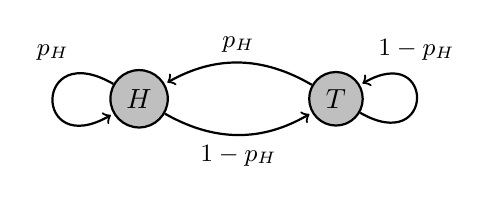
\begin{tikzpicture}[->,shorten >=1pt,auto,node distance=3cm,
    thick,main node/.style={circle,draw,font=\sffamily\Large\bfseries}]

\node[fill=gray!50, circle, draw=black] (H) at (0,0) {$H$};
\node[fill=gray!50, circle, draw=black] (T) at (2.5,0) {$T$};

\path[every node/.style={font=\sffamily\small}]
(H) edge [in=210,out=150, loop] node[above=10pt] {$p_H$} (H)
(H) edge [bend right] node[below] {$1-p_H$} (T)
(T) edge [bend right] node[above] {$p_H$} (H)
(T) edge [in=30,out=330, loop] node[above=10pt] {$1-p_H$} (T);

\end{tikzpicture}

\chapter{Conclusion} \label{chap:conclusion}


\chapter{Acknowledgements} \label{chap:acknowledgements}


\clearpage
\chapter*{Declaration of Authorship}

I hereby solemnly declare, by my own signature, that I have independently authored the presented work and have not used any sources or aids other than those indicated. All passages taken verbatim or in content from the specified sources are identified as such.

I consent to the archiving of this Bachelor thesis.

\hfill
\vspace{2cm} Innsbruck, \findate \hfill Lukas Prader \includegraphics[height = 10mm]{"signature.png"}


\newpage
\printbibliography[]
\newpage
\appendix



\end{document}